  % Use only LaTeX2e, calling the article.cls class and 12-point type.

\documentclass[12pt]{article}

% Users of the {thebibliography} environment or BibTeX should use the
% scicite.sty package, downloadable from *Science* at
% www.sciencemag.org/about/authors/prep/TeX_help/ .
% This package should properly format in-text
% reference calls and reference-list numbers.

\usepackage{scicite}

% Use times if you have the font installed; otherwise, comment out the
% following line.

\usepackage{times}

\usepackage{graphicx}
\usepackage{hyperref}

% The preamble here sets up a lot of new/revised commands and
% environments.  It's annoying, but please do *not* try to strip these
% out into a separate .sty file (which could lead to the loss of some
% information when we convert the file to other formats).  Instead, keep
% them in the preamble of your main LaTeX source file.


% The following parameters seem to provide a reasonable page setup.

\topmargin -1.5cm
\oddsidemargin 0.0cm
\textwidth 16cm 
\textheight 23.5cm
\footskip 1.0cm

%The next command sets up an environment for the abstract to your paper.

\newenvironment{sciabstract}{%
\begin{quote} \bf}
{\end{quote}} 

% If your reference list includes text notes as well as references,
% include the following line; otherwise, comment it out.

%\renewcommand\refname{References and Notes}

% The following lines set up an environment for the last note in the
% reference list, which commonly includes acknowledgments of funding,
% help, etc.  It's intended for users of BibTeX or the {thebibliography}
% environment.  Users who are hand-coding their references at the end
% using a list environment such as {enumerate} can simply add another
% item at the end, and it will be numbered automatically.

\newcounter{lastnote}
\newenvironment{scilastnote}{%
  \setcounter{lastnote}{\value{enumiv}}%
  \addtocounter{lastnote}{+1}%
  \begin{list}%
  {\arabic{lastnote}.}
  {\setlength{\leftmargin}{.22in}}
  {\setlength{\labelsep}{.5em}}
}
{\end{list}}

\title{Assignment 1} 

\author
{Filipe Pires [85122], João Alegria [85048]\\
\\
Information Retrieval\\
\normalsize{Department of Electronics, Telecommunications and Informatics}\\
\normalsize{University of Aveiro}\\
} 

\date{\today{}}

%%%%%%%%%%%%%%%%% END OF PREAMBLE %%%%%%%%%%%%%%%%

\begin{document} 

% Double-space the manuscript.

\baselineskip18pt

% Make the title.

\maketitle 

% Place your abstract within the special {sciabstract} environment.

%\begin{sciabstract}
  
%\end{sciabstract}

% In setting up this template for *Science* papers, we've used both
% the \section* command and the \paragraph* command for topical
% divisions.  Which you use will of course depend on the type of paper
% you're writing.  Review Articles tend to have displayed headings, for
% which \section* is more appropriate; Research Articles, when they have
% formal topical divisions at all, tend to signal them with bold text
% that runs into the paragraph, for which \paragraph* is the right
% choice.  Either way, use the asterisk (*) modifier, as shown, to
% suppress numbering.

\section*{Introduction}

This report aims to describe the work developed for the first assignment
of the discipline of 'Information Retrieval', explaining the overall
processing pipeline.
We include a short description of each class developed and of the respective
methods, as well as the instructions on how to run our code.

The program implemented in Python version 3 has the purpose of indexing
documents given as input in a compressed format.
This document indexer consists of a corpus reader, a tokenizer and the 
actual indexer.

Along with the description of the solution, we also answer to a few questions
proposed for the assignment \cite{assign1}.

All code and documentation is present in our public GitHub at 
\newline \url{https://github.com/joao-alegria/RI}.

\newpage
\section*{1. Architecture}

In order to maintain a modular architecture, we resorted to the Python library 
{\it Abstract Base Classes\/} (or simply ABC) \cite{abclib}.
This module provided us with the infrastructure for defining abstract classes
for each of our own modules.
As seen in Fig.\ref{fig:classdiagram}, the 3 base classes all derive from 
an ABC.

The choice of this form of architecture was due to several reasons: modules
allow the reduced coupling between system components, making it easy to replace
or add new ones; creating variations of the solution (as we will see on the
\texttt{Tokenizer} class) becomes far simpler and easier to manage; adopting this 
program structure also helps making the extension/adaptability of the 
program to other corpora structures easier to implement.

\begin{figure}[h!]
  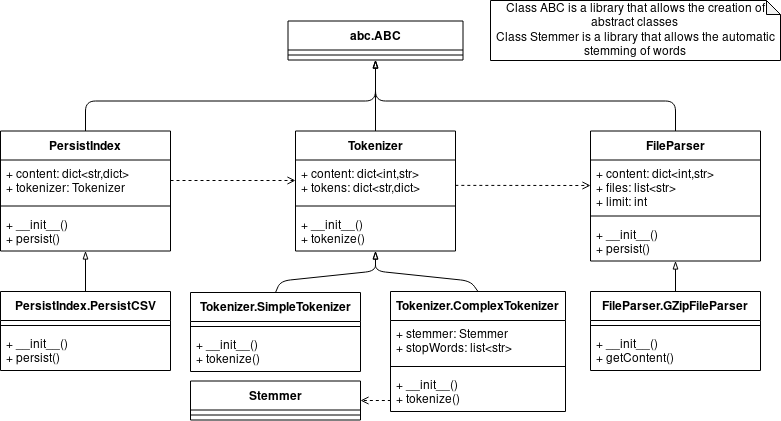
\includegraphics[width=\linewidth]{ClassDiagram.png}
  \caption{Program's class diagram.}
  \label{fig:classdiagram}
\end{figure}

The class \texttt{FileParser} is an abstract class for all file parsers.
In our case, we only needed to develop 1 derived class to parse files on
.gz format. 
It is \texttt{GZipFileParser} that actually reads the various compressed 
files passed to the program and dinamically processes them, meaning that
the program decompresses the file line by line to retrieve the text bytes 
and then creates a dictionary that makes direct relation between a document 
id("PMID") and it's title("TI").
To improve our reading performance we used a reading buffer that 
significantly decreases the execution time. 

\newpage
\texttt{Tokenizer} is the abstract base class for our 2 Tokenizer 
implementations.
The \texttt{SimpleT} \texttt{okenizer} contains only one method called 
{\it tokenize()\/}, defined by the parent, that receives some text and processes it by replacing all non-alphabetic 
characters by a space, lowercases the entire content, splits on whitespace, 
and ignores all tokens (all resulting strings after the split operation) with 
less than 3 characters.
The \texttt{ComplexTokenizer}, on the other hand, is, as the name indicates, a
more complex implementation aimed to return a more valuable set of tokens.
This class integrates a stopword filter to ignore words considered not relevant
and a stemmer to standardize all words, i.e. it normalizes the terms (or tokens)
according to an algorithm that considers the English language by conflating
words with the same linguistic base form.
The stemmer used was PyStemmer \cite{pystemmer}, which is an implementation of 
Porter Stemmer, as recommended on the assignment instructions. 
For this reason, our Complex Tokenizer depends on the class \texttt{Stemmer}.
In addition this tokenizer also implements custom rules conserning puctuation
and more.
We opted to implement restrictions in a way that maintains dates, emails, phone
numbers, money amounts and numbers in general, but eliminate any kind of 
regular punctuation and separates words connected with hyphens or underscores,
considering the resulting terms as tokens as well.

\texttt{Indexer} is the abstract base class that serves as the interface for any
indexer that may be implemented. In our case we only needed to implement 1, 
which is present in \texttt{FileIndexer}. 
Our Indexer depends on the FileParser and the Tokenizer, because it needs the 
content from the files and it needs to know the tokenization strategy chosen,
having that the program can successfully construct the whole index, which is
basically the IDs of the documents where a given token appears and the number 
of occurrences in each of those documents, for all of the tokens from the 
entire vocabulary of the input files.

Finally we have the \texttt{PersistIndex} abstract class that only depend on 
the \texttt{Indexer}.
Our implementation, \texttt{PersistCSV}, is the class responsible for 
persisting the index in plaintext.
This is done by storing the data present in a dictionary constructed by one 
of the previous tokenizers in a text file using the method {\it persist()\/}. 
To try to improve our performance we adopted an batch processing like system, 
were we store the token, all the document ID's where it appeared and the 
numbers of occurences on each document at the same time. 
After testing we observed that this approach improve our performance and 
execution time.

\newpage
\section*{2. Data Flow}

The file \texttt{CreateIndex.py} serves as the command to be executed in order to 
indexing all documents passed as arguments.
This command has the following format:

\begin{quote}
\begin{verbatim}
$ python3 CreateIndex.py [-h] [-o outputFile] [-l limit] \\
  [-t tokenizer] inputFile1 [inputFile2]+
\end{verbatim}
\end{quote}

Here, \texttt{-h} is the option that presents the manual for the command usage.
Options \texttt{-o} and \texttt{-l} allow the definition of the output file's 
name and of the limit for the number of lines to be processed in each input file.
Option \texttt{-t} makes possible for the user to choose the type of tokenizer
to be used, and the alternatives are: 'simple' for the use of the 
\texttt{SimpleTokenizer} class, and 'complex' for the \texttt{ComplexTokenizer} class.
The previous arguments are all optional and the actual values for these arguments
must appear right after the respective options.
The final argument(s) of the command must be the name(s) of the input file(s) to
be indexed.

Once the arguments are validated, the program passes the file name(s) to the 
File Parser, already capable of processing multiple files. 
Once the parsing process is completed, the chosen Tokenizer accesses the 
data and tokenizes everything, that in this case is the title of each 
document.
Lastly, the information created by the tokenizer - the actual index - is 
persisted into an output file, making possible its consultation and analysis.

Below we present both implementations of the method {\it tokenize()\/} for
comparison purposes.

\begingroup
\addtolength\leftmargini{-0.4in}
\addtolength\baselineskip{-0.05in}
\begin{quote}
\begin{verbatim}
  def tokenize(self, processText): # of class SimpleTokenizer
    tokens=self.regex2.split(self.regex1.sub(" ", 
                                          processText.lower()))
    return [t for t in tokens if len(t) >= 3]

  def tokenize(self, processText): # of class ComplexTokenizer
    intermidiateTokens = self.regex1.split(processText.lower())
    resultingTokens = []
    for t in intermidiateTokens:
        t = self.regex2.sub(" ", t) if self.regex3.search(
            t) else self.regex4.sub(" ", t)
        additionalWords=list(filter(None,self.regex1.split(t)))
        if len(additionalWords) == 0:
            continue
        resultingTokens += additionalWords
    return [t for t in self.stemmer.stemWords(resultingTokens) 
      if t not in self.stopWords and len(t) > 2]
\end{verbatim}
\end{quote}
\endgroup

\newpage
\section*{3. Discussion}

To test the capabilities of the developed software, we indexed 2 large 
compressed files made available along with the assignment description
with the names \texttt{2004\_TREC\_ASCII\_MEDLINE} \texttt{\_1.gz} and 
\texttt{2004\_TREC\_ASCII\_MEDLINE\_2.gz}.
Each file is a collection (corpus) of documents.
In this chapter we discuss our implementation's performance over these 
files and answer the following questions:

a) What is the total indexing time and final index size on disk?

b) What is the vocabulary size?

c) What are the ten first terms (in alphabetic order) that appear in 
only one document (document frequency = 1)?

d) What are the ten terms with highest document frequency?

To answer question a), we simple added the command \texttt{time} in the
beginning of the execution of the \texttt{CreateIndex.py} 
(e.g. \texttt{\$time python3 CreateIndex.py (...)}).
This command returned us 3 measured times during the execution, but we 
were interested only in one of them - the Elapsed real time (in seconds)
since the execution start.
After all code optimizations, the best value we could achieve was of 
\texttt{5'40''} (six minutes and ten seconds) and an index size on 
disk of \texttt{436,1 Mbs} with the \texttt{SimpleTokenizer} and of 
\texttt{10'22''} (ten minutes and fifty-two seconds) and an index 
size on disk of \texttt{383.7 Mbs} with the \texttt{ComplexTokenizer}.

For the remaining questions, we developed a small script called
\texttt{IndexAnalyzer.py} that processes the output file passed as argument.
The calculated size of the vocabulary generated by the Simple Tokenizer
was \texttt{346221} unique terms and of the vocabulary generated by the 
Complex Tokenizer was \texttt{342949}.

The 10 first terms (ordered alphabetically) with document frequency of 1 
of the Simple and Complex Tokenizers are the following:

\begingroup
\addtolength\leftmargini{-0.4in}
\addtolength\baselineskip{-0.05in}
\begin{quote}
\begin{verbatim}
Simple:
'aaaat', 'aaab', 'aaac', 'aaacr', 'aaact', 'aaaction', 'aaad', 
'aaaga', 'aaagat', 'aaah'

Complex:
'$102', '$105m', '$108m', '$10m', '$11', '$111k', '$115',
'$121', '$125', '$13'
\end{verbatim}
\end{quote}
\endgroup

These were retrieved first filtering out all terms with document frequency
above 1 and then ordering the remaining tokens alphabetically with the use 
of the {\it quicksort\/} algorithm as a safe measure, although we store 
the indexes alphanumerically by default.

\newpage
The 10 terms with highest document frequency (for both tokenizers) are the 
following:

\begingroup
\addtolength\leftmargini{-0.4in}
\addtolength\baselineskip{-0.05in}
\begin{quote}
\begin{verbatim}
Simple:
Terms: 'and'(2044099), 'the'(2033707), 'with'(633062), 
'for'(608296), 'from'(234101), 'patients'(228824),
'human'(217457), 'cell'(184034), 'cells'(174998),
'study'(170588)

Complex:
Terms: 'cell'(359036), 'patient'(289130), 'effect'(281633),
'human'(232049), 'studi'(219451), 'activ'(202904),
'protein'(188952), 'use'(178166), 'rat'(173397),
'diseas'(169893)
\end{verbatim}
\end{quote}
\endgroup

To retrieve these terms, we stored the maximum number of occurrences
during the output file's reading process and then search for the terms
with that document frequency; if these terms are less than 10, we proceed 
on filtering for documents with the following highest frequency
and repeat the process until the 10 terms are found. \\

Let us now take a closer look at these results.
Starting with the indexing time, the indicated values were the minimum
achievable after optimizing our code as much as we could.
These execution times were reduced mainly due to the use of a Buffer Reader
and of batch writings to the output file.
The achieved sizes on disk of the indexes were the outcome of our way of 
treating the data. 
By balancing the data normalization and reducing the lost of 
knowledge throughout the processing pipeline, our solution seems to 
deliver indexes of considerably good value.
This space is smaller for the Complex Tokenizer as it is able to remove
unnecessary characters and compress the data in a smarter way.

The reason for the answers to questions b) and c) to be different depending on 
the tokenizer used is simple to understand by looking at their implementation.
For example, as the \texttt{ComplexTokenizer} splits tokens by hyphens, this
alone will already increase the vocabulary for the respective index.
Another example with this tokenizer is that we decided it should not eliminate
some symbols from words and, when these symbols occur in the beggining of a 
word, they are sorted as words that appear before the letter 'a', altering,
in consequence, the answer to question c).

Again, for the answers to the final question, the tokenizer implementations
alter the results as they treat specific words in different ways.
For example, the \texttt{ComplexTokenizer} eliminates stopwords such as 'and'
that occur massively in most English texts.

\newpage
\section*{Conclusions}

After completing the assignment, we drew a few conclusions regarding our
solutions and the whole concept of indexing files containing textual information.

First of all, we had to learn how to deal with the actual tokenization of 
words and what rules should be taken in consideration when normalizing them.
In this sense, the delivered code is the result of this learning process.

Second, a few unpredicted setbacks such as the extensive time that Python 
took when reading the input files without a buffer in the middle, made us 
realize more clearly the fact that, when dealing with large amounts of data,
the traditional tools are usually insufficient and that we must look at the 
challenges with a different perspective.

Regarding our satisfaction with the delivered code, not much can be said
since we did not have access to the answers considered 'more correct'.
However, taken in consideration the guidance given by our professor for 
the average execution time, and looking at a few results shared by other 
class colleagues, we believe that our solution fulfills all task requirements
and surpasses the expectations in terms of performance.

\begin{thebibliography}{9}
  \bibliographystyle{Science}

  \bibitem{assign1}
    S. Matos,
    \textit{IR: Assignment 1},
    University of Aveiro,
    2019/20.
  \bibitem{abclib}
    Abstract Base Classes,
    Python.org,
    \textit{https://docs.python.org/2/library/abc.html},
    (visited in 01/10/2019)
  \bibitem{pystemmer}
    Snowball Stem PyStemmer,
    GitHub.com,
    \textit{https://github.com/snowballstem/pystemmer},
    (visited in 01/10/2019)
  
\end{thebibliography}

\clearpage

\end{document}




















